\documentclass{utap}

\usepackage{wrapfig}
\usepackage{xepersian}

\graphicspath{{./img/}}

\title{تمرین  بازسازی کد}
\author{
    \href{mailto:bardia.eghbali@gmail.com?subject=[AP\%20S98\%20Refactoring]\%20}{بردیا اقبالی},
    \href{mailto:ahhabibvand@gmail.com?subject=[AP\%20S98\%20Refactoring]\%20}{امیرحسین حبیب‌وند}
}
\course{برنامه‌سازی پیشرفته}
\deadline{جمعه ۱۶ فروردین ۱۳۹۸، ساعت ۲۳:۵۵}
\lecturer{رامتین خسروی}
\lstset{
    numbers=left,
    frame=leftline,
}

\newcommand{\chap}[1]{\hfill\normalfont\normalsize فصل #1}

\begin{document}
\maketitle

\section{بازسازی}
تعاریف زیادی از
«کد تمیز»\LTRfootnote{clean code}
وجود دارد؛ اما احتمالاً یکی از بهترین تعریف‌ها متعلق به
«بیارنه استروستراپ»\LTRfootnote{Bjarne Stroustrup}
خالق و توسعه‌دهنده‌ی زبان \lr{C++} است. وی در تعریف خود از کد تمیز، دو مورد را به عنوان معیار‌های اساسی تمیزی کد برمی‌شمارد:
\begin{itemize}
\item
منطق و الگوریتم کد باید آن‌قدر واضح و قابل‌فهم باشد که اشکالات و نقص‌های ﺟﺰﺋﯽ نتوانند از چشم برنامه‌نویس و آزمونگر کد دور بمانند. ضمن این که وضوح کد باید به حدی بالا باشد که برنامه‌نویس را از نوشتن یادداشت (کامنت\LTRfootnote{comment}) بی‌نیاز کند.

\item
کارایی\LTRfootnote{performance}
برنامه‌ی نوشته‌شده باید در بهینه‌ترین\LTRfootnote{optimal}
شکل ممکن باشد تا بعدها برنامه‌نویس دیگری به بهانه‌ی بهینه‌سازی\LTRfootnote{optimization}
برنامه‌ی سابق با ایجاد تغییرات نادرست سبب نامنظم~شدن و کثیف~شدن کد نشود.
\end{itemize}

در عمل، در اکثر مواقع شما بعد از یک طراحی نسبتاً خوب و پیاده‌سازی آن، برای مدتی طولانی از آن کد برای هدف خود استفاده می‌کنید و در طول این مدت تغییراتی در آن ایجاد می‌کنید و قابلیت‌های زیادی را به آن می‌افزایید.

\begin{wrapfigure}[13]{L}{0.4\textwidth}
    \centering
    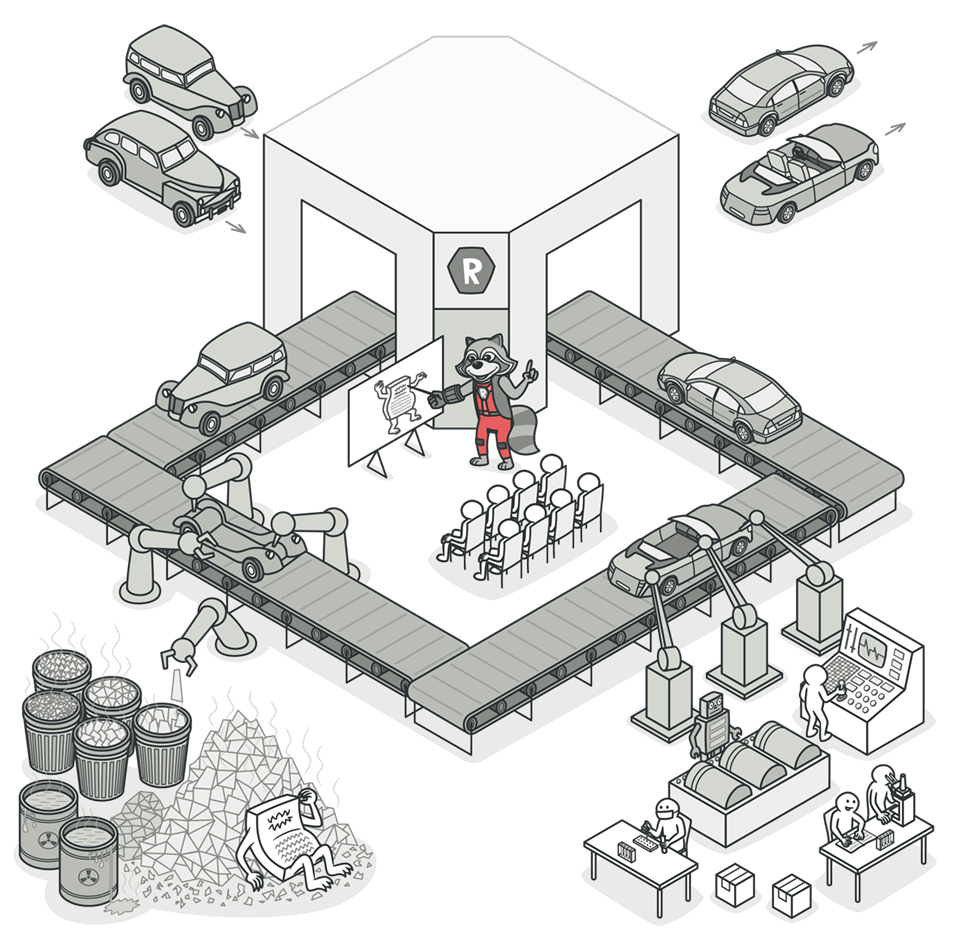
\includegraphics[width=0.4\textwidth]{refactoring}
\end{wrapfigure}

پس از مدتی نه‌چندان طولانی، این تغییرات باعث می‌شوند که شما دیگر عملکرد کد را به‌وضوح متوجه نشوید و به~تبع آن، توانایی تغییر و ارتقای کد را نیز از دست می‌دهید. همین زنجیره‌ی اتفاقات به ظاهر ساده در تاریخچه‌ی نسبتاً کوتاه توسعه‌ی نرم‌افزاری باعث نابود~شدن شرکت‌های بسیاری در این عرصه شده است.

حال با توجه به خطرات و مشکلاتی که یک کد کثیف به همراه دارد، باید راه‌حلی برای رفع کثیف‌بودن کد و جلو‌‌گیری از ایجاد آن ارائه دهیم. شما در این تمرین کامپیوتری با روند \textit{بازسازی}\LTRfootnote{refactoring} کد آشنا می‌شوید.

\textit{بازسازی} عملیاتی است که در طی آن ساختار یک نرم افزار به صورتی تغییر و بهبود می‌یابد که بدون از دست‌رفتن کارآیی‌ها و تغییر رابط کاربری\LTRfootnote{interface} برنامه، ساختار درونی کد به طرز قابل توجهی تمیزتر می‌شود.

بنیادی‌ترین مفهوم یاری‌کننده‌ی یک برنامه‌نویس در طی عملیات بازسازی شناخت عناصری است که باعث کثیف شدن کدها می‌شوند و به اصطلاح به آن‌ها \lr{code smell} گفته می‌شود.

در این تمرین از شما انتظار می‌رود کدی را که برای تمرین اول نوشته‌اید بازسازی کنید؛ بنابراین \textbf{خوانایی و تمیز~بودن کد} در این تمرین بیشترین اهمیت را دارد. در ادامه توضیحاتی درباره‌ی بازسازی کد ارائه می‌شود. پیشنهاد می‌کنیم که ابتدا صورت این تمرین را به طور کامل مطالعه کنید و سپس بازسازی کد خود را شروع کنید.

\section{کد تمیز}
عواملی در کد وجود دارند که ممکن است باعث کثیف~شدن آن شوند؛ در ادامه برخی از این عوامل توضیح داده شده‌اند. توجه کنید که در انتهای این تمرین نمره‌ی شما فقط بر اساس عوامل زیر سنجیده می‌شود و به~ازای هر یک از موارد زیر که در کد شما وجو داشته باشد نمره‌ی شما کاسته خواهد شد. ساختار کلی کد و طراحی شما نباید تغییر کند و فقط ساختار درونی آن می‌تواند تغییر کند.

این عوامل خلاصه‌ای از کتاب \lr{Clean Code}\LTRfootnote{Robert C. Martin. 2008. Clean Code: A Handbook of Agile Software Craftsmanship (1 ed.). Prentice Hall PTR, Upper Saddle River, NJ, USA.} هستند. عبارت مقابل هر بخش شماره‌ی فصل مرتبط با آن بخش را در کتاب نشان می‌دهد.
نسخه‌ی الکترونیکی این کتاب در سایت درس قابل دسترسی است.

\subsection[نام‌گذاری]{نام‌گذاری\chap{۲}}
\begin{itemize}
    \item
استفاده از نام‌های نامرتبط کار درستی نیست. مثلاً استفاده از متغیر‌هایی با نام‌های \lr{a} و \lr{b} که هیچ توضیحی ارائه نمی‌دهند و خواننده را گیج می‌کنند. (فصل ۱۷، \lr{N1})
    \item
نام متغیر باید کاربرد و مکان استفاده از متغیر را نشان دهد.
اسامی کلاس‌ها\LTRfootnote{classes}، ساختارها\LTRfootnote{structures} و اشیا\LTRfootnote{objects} باید عبارت‌های اسمی\LTRfootnote{noun phrase} باشند. اسامی کلاس‌ها و اشیا باید با حرف بزرگ\LTRfootnote{capital} شروع شوند؛ مانند: \lr{Customer} و \lr{Account}.
    \item
نام تابع باید وظیفه‌ی تابع و تأثیرات جنبی\LTRfootnote{side-effects} احتمالی تابع بر محیط را توضیح دهد.
اسامی توابع باید عبارت‌های امری\LTRfootnote{verb phrase} باشند و با حرف کوچک شروع شوند؛ مانند: مثل \lr{get}, \lr{set} و \lr{deletePage}.
\end{itemize}

\subsection[توابع]{توابع\chap{۳}}
  \begin{itemize}
	\item
یک تابع باید یک کار انجام دهد، آن را خوب انجام دهند و فقط همان کار را انجام دهند.
    \item
توابع باید تا حد امکان \textbf{کوتاه} باشند.
% تابع باید حداکثر ۶ (۸‌؟) خط باشد.         [منبع؟]
طول توابع به‌ندرت باید به ۲۰ خط برسد.
	\item
هر تابع باید حداکثر به یک سطح پایین‌تر دسترسی داشته باشد؛ مثلاً حرکت با یک حلقه روی لیستی از اشیا و تغییر ویژگی‌\LTRfootnote{property}های هر کدام از اشیا دسترسی به دو سطح پایین‌تر از تابع است. و این عملیات باید در تابعی جداگانه پیاده‌سازی شود.
	\item
تعداد آرگومان‌های تابع تا حد امکان کم (حداکثر ۳ تا) باشد.
گاهی می‌توان از آرگومان‌هایی از نوع اشیا یا ساختارها برای بسته‌بندی چند آرگومان مرتبط و کاهش تعداد آرگومان‌های توابع استفاده کرد؛ مثلاً به جای دو متغیر از نوع \lr{\lstinline{double}} از یک شیء از نوع \lr{\lstinline{Point}} استفاده کنیم.
    \item
آرگومان‌های تابع نباید به عنوان خروجی تابع استفاده می‌شوند.
یک تابع فقط باید بتواند از طریق مقدار بازگشتی خود بر محیط بیرون تأثیر بگذارد و نباید از طریق تغییر آرگومان‌ها بر محیط تأثیری داشته باشد. (فصل ۱۷، \lr{F2})
    \item
استفاده از پرچم\LTRfootnote{flag}‌ها (معمولاً آرگومان از نوع بولی\LTRfootnote{boolean}) برای تعیین نحوه‌ی عملکرد تابع کار درستی نیست.
مثالی از این کار ارسال یک متغیر به نام \lr{flag} به تابع فقط برای اجرای یک بخش کد در حالتی خاص است. چنین تابعی در واقع دو تابع مختلف است که باید به صورت جدا از هم پیاده‌سازی شوند و در زمان مناسب فراخوانی\LTRfootnote{Call} شوند. (فصل ۱۷، \lr{F3})
    \item
انجام بیش از یک کار در یک تابع درست نیست. هر تابع باید فقط یک کار را انجام دهد و این کار را به شیوه درستی پیاده و اجرا کند. همچنین نباید در کنار انجام این کار تأثیری در متغیرها و دیگر اجزای برنامه داشته باشد. (فصل ۱۷، \lr{G30})
    \end{itemize}

\subsection[قالب‌بندی]{قالب‌بندی\LTRfootnote{formatting}\chap{۵}}
  \begin{itemize}
        \item
\textbf{دندانه‌گذاری}\LTRfootnote{indentation}
در کد اهمیت بالایی دارد و حتماً هر محدوده\LTRfootnote{scope} باید یک دندانه داخل‌تر باشد. همچنین هر تابع باید حداکثر یک یا دو دندانه داخل رفته باشد.
	\item
در نام‌گذاری توابع و متغیر‌ها باید از یک روش واحد نام‌گذاری\LTRfootnote{naming convention} استفاده شده باشد؛ مثلاً یا همه‌ی متغیر‌ها به صورت \lr{CamelCase} نام‌گذاری شده باشند یا همه به شکل \lr{snake\_case}. در هر صورت، دیگر قوانین نام‌گذاری نیز باید رعایت شوند.
    \item
\textbf{ثبات}\LTRfootnote{consistency} یکی دیگر از نکات مهم در کد~نویسی است. سعی کنید که همیشه از یک الگو و روند در پیاده‌سازی و نام‌گذاری‌های خود استفاده کنید. (فصل ۱۷، \lr{G11})
    \end{itemize}

\subsection[یادداشت‌ها]{یادداشت‌ها (کامنت\LTRfootnote{comment}‌ها)\chap{۴}}
	  \begin{itemize}
	        \item انواع یادداشت
            در این تمرین استفاده از یادداشت (کامنت) به هیچ نحوی قابل قبول نیست.
	    \end{itemize}
برای آشنایی بیشتر با یادداشت‌های مفید و مضر به فصل ۴ کتاب مراجعه کنید.

\subsection[مشکلات دیگر]{مشکلات دیگر\chap{۱۷}}
اشکالات دیگری نیز ممکن است در کد شما دیده شود که باید آن‌ها را برطرف کنید:
	  \begin{itemize}
        \item \textbf{کد تکراری}\LTRfootnote{duplication}:
از مهم‌ترین نکاتی که باید در این تمرین رعایت کنید، جلوگیری از تکرار کد است و کد تکراری به هیچ وجه قابل قبول نیست. (\lr{G5})
		\item \textbf{کدهای مرده}\LTRfootnote{dead codes}:
کدهایی که دیگر در هیچ قسمتی از برنامه فراخوانی نمی‌شوند نباید در متن برنامه وجود داشته باشند. (\lr{G9})
		\item استفاده از اعداد جادویی\LTRfootnote{magic numbers}:
اعداد و ثابت‌ها نباید به طور مستقیم در کد استفاده شوند و باید در متغیر‌های ثابت ذخیره شوند و از این متغیر‌ها در کد استفاده شود. مثلاً عدد $\pi$ را باید در ابتدای برنامه در متغیری به نام \lr{PI} ذخیره کنیم و از این ثابت در بقیه کد استفاده کنیم. (\lr{G25})
	   \end{itemize}
\section{نکات پایانی}
	  \begin{itemize}
        \item
هدف این تمرین بازسازی کد خودتان است و نباید ساختار کلی و طراحی شما تغییر کند.
		\item
کد نهایی شما با موارد آزمون تمرین ۱ نیز آزموده خواهند شد و برای این قسمت نمره‌ای در نظر گرفته شده است.
موارد آزمون تمرین ۱ را می‌توانید از سایت درس دریافت کنید.
		\item
یک نمونه از بازسازی کد را می‌توانید در \dots{} مشاهده کنید.  % @ToDo

	  \end{itemize}

\section{نحوه‌ی تحویل}
    پرونده‌ی\LTRfootnote{file} برنامه‌ی خود را با نام \lr{R-SID.cpp} در صفحه‌ی \lr{CECM} درس بارگذاری کنید که \lr{SID} شماره‌ی دانشجویی شماست؛ برای مثال اگر شماره‌ی دانشجویی شما ۸۱۰۱۹۷۹۹۹ باشد، نام پرونده‌ی شما باید \lr{R-810197999.cpp} باشد.
    \begin{itemize}
        \item
برنامه‌ی شما باید در سیستم‌عامل لینوکس و با مترجم \lr{g++} با استاندارد \lr{\texttt{c++11}} ترجمه و در زمان معقول برای ورودی‌های آزمون اجرا شود.
        \item
در این تمرین اجازه‌ی استفاده از مفاهیم شیءگرایی را \textbf{ندارید}.
        \item
از صحت قالب\LTRfootnote{format} ورودی‌ها و خروجی‌های برنامه‌ی خود مطمئن شوید. توجه کنید که آزمون خودکار برنامه به \textbf{تعداد و محل فاصله‌ها و خطوط خالی} نیز حساس است. توصیه می‌کنیم حتماً برنامه‌ی خود را با ورودی و خروجی نمونه بیازمایید و از ابزارهایی مانند \lr{\texttt{diff}} برای اطمینان از درستی عملکرد برنامه‌ی خود برای ورودی نمونه استفاده کنید.
        \item
هدف این تمرین یادگیری شماست. لطفاً تمرین را خودتان انجام دهید. در صورت کشف تقلب مطابق قوانین درس با آن برخورد خواهد شد.
    \end{itemize}
\end{document}
